\documentclass[]{article}
\usepackage{amssymb,amsmath}
\usepackage{graphicx}
\usepackage{hyperref}
\usepackage{natbib}
\bibliographystyle{plainnat}

\title{Iron-Oxide Exsolution an Important Power Source for Earth's Dynamo}

\author{Nicholas Knezek
	\and Tushar Mittal
	\and Chris McGuire 
	\and Sarah Arveson
	\and Curtis Williams 
	\and Jackie Li}
\date{}

\begin{document}
	\maketitle
	
	\section{Abstract}\label{abstract}
	Earth has been observed to have a global magnetic field for at least the past 3.5 billion years \citep{Tarduno2015}, but recent high thermal conductivity measurements \citep{Pozzo2012} and resulting young inner-core ages \citep{Labrosse2015} make it difficult to sustain Earth's magnetic field by cooling and inner-core growth alone. Exsolution of light elements such as magnesium \citep{Badro2016,ORourke2016a} and silicon \citep{Hirose2017} from Earth's core have been proposed as sources of energy to resolve this problem. We integrate these solubility measurements into a unified system to show that exsolution of iron-oxide from the core is an important third source of energy for the dynamo. We create a coupled thermodynamic evolution and chemical interaction model between Earth's core and mantle and show that exsolution of light elements from the core depends heavily on the composition of the background mantle and timescale of mantle convection. We show iron-oxide exsolution is the dominant source of compositional entropy production across a range of plausible parameter choices, with possible implications for the origin of LLSVPs and ULVZs.  We also find exsolution reduces the magnitude of increase in available entropy at inner-core nucleation and allows for a wider range of inner-core nucleation times when compared to dynamos powered by cooling, making detection of a paleomagnetic signal of inner-core nucleation more difficult. 
	
	\section{Introduction}\label{introduction}
	
	
	TUSHAR - I'll deal with this section ..
	
	\section{Model}\label{model}
	We model the thermal evolution of the Earth using a coupled core-mantle
	thermodynamic model following the methods of \citet{Stevenson1983} for
	parameterized mantle convection and \citet{Nimmo2015} for core
	thermodynamics. We add chemical reactions between the core and mantle to
	this system, modeled as a set of equlibrium reactions between the core and a thin interaction layer at the base of the mantle. This layer is then removed over time by background mantle convection, bringing fresh material in contact with the core. These reactions govern the exsolution of light elements from the core into the mantle, which contribute to the heat and entropy budget of the core in the thermal model. This system is cast as a system of first-order ODEs and solved forward in time from Earth's formation to the present day.
	
	\subsection{Chemical Interactions}\label{chemical-interaction-layer}
	We model chemical interactions between the core and mantle as a system of equilibrium reactions with the base of the lower mantle. First-principles calculations and seismic observations argue for a pyrolitic lower mantle, necessitating the convesion of minerals such as olivine and ferropericlase transported from the upper mantle into Bridgemanite at depth. While the exact mechanisms of this process are not well understood, it requires interaction between mineral species at relatively large distances over timescales of millions of years. Thus, at long enough timescales the chemical state of the lower mantle should be able to be modeled as an equilibrium reaction system.
	
	A similar argument can be made about core-mantle interactions. Material from the lower mantle can both diffuse into and exolve out of the core, setting up a system of equlibrium reactions. To model this, we assume a typical length-scale for chemical interactions in the mantle and keep track of the moles of each mantle mineral in this layer. There is considerable uncertainty concerning the mechanisms by which Earth's core and mantle interact, and therefore the appropriate length-scale is uncertain. If chemical interaction is dominated by atomic diffusion, interaction length-scales of H$\sim$1-10m over 100 Myr may be appropriate \citet{Bina2010,VanOrman2003}. If grain-boundary diffusion occurs at the CMB, it could allow H$\sim$100m \citet{Hayden2007}, while H$\sim$1km could be appropriate if core material physically intrudes into the lower mantle \citep{Kanda2006}.
	
	In our model, we track Fe, Mg, Si, O in the core. These species exchange with the mantle through the equilibrium reactions
	\begin{align}
	MgO (mantle) &\leftrightarrow Mg^{(met)} + O^{(met)} \label{eq:m1}\\
	SiO_2 (mantle) &\leftrightarrow Si^{(met)} +2 O^{(met)}\label{eq:m2}\\
	FeO (mantle) &\leftrightarrow Fe^{(met)} +O^{(met)}\label{eq:m3}
	\end{align}
	as can be seen in figure 1. Each of these reactions is governed by their temperature dependent equilibrium constant. We use the values reported by \citep{Hirose2017} for SiO2 and FeO and \citep{Badro2016} for MgO. 	In our model, we only allow Mg, Si, and O to leave the core, but not enter. An undersaturated core would allow light elements from the mantle to dissolve into the core fluid at the CMB. However, this would form a thin stratified layer at the CMB heavily enriched in light elements which would not easily mix with the bulk of the core and would shut down further dissolution of material [CITE]. Thus, the bulk of the core composition would remain unchanged.
	
	The composition of the mantle interaction layer consists of MgO,
	SiO\(_2\), FeO, MgSiO\(_3\), and FeSiO\(_3\). The total number of moles
	of each species are tracked and governed by the reactions
	\begin{align}
	MgSiO_3 &\leftrightarrow MgO + SiO_2\label{eq:c1}\\
	FeSiO_3 &\leftrightarrow FeO + SiO_2\label{eq:c2}\\
	FeSiO_3 + MgO &\leftrightarrow FeO + MgSiO_3\label{eq:c3}
	\end{align}	
	where the third reaction maintains stoichiometry in the layer and has an
	equilibrium constant defined as 1. This constrains \(K_\eqref{eq:c1}\) to equal
	\(K_\eqref{eq:c2}\). The lower mantle is expected to be mostly Bridgemanite in the present day, so that $K_\eqref{eq:c1} = K_\eqref{eq:c2}  \ll 1$.
	
	\subsection{Interaction Layer Dynamics}
	Exsolved material from the core builds up at the base of the mantle over time,
	altering the composition of the interaction layer and therefore
	affecting the exsolution of core species. At the same time,
	the interaction layer moves with the background mantle convection along the free
	surface of the CMB, setting up a ``conveyer belt'' system as in figure
	1. In this system, the layer is removed by mantle upwellings or plumes
	and replaced with fresh background mantle due to downwellings or sinking
	slabs on a timescale \(\tau\) set by the background mantle convection.
	Analytical stability analyses and 2D numerical mantle convection codes
	show that exsolved material in our model never reaches the
	required thickness and buoyancy contrast to form Rayleigh-Taylor
	instabilities, in contrast with other recent results \citep{Helffrich2017}.
	
	\begin{figure}\centering
		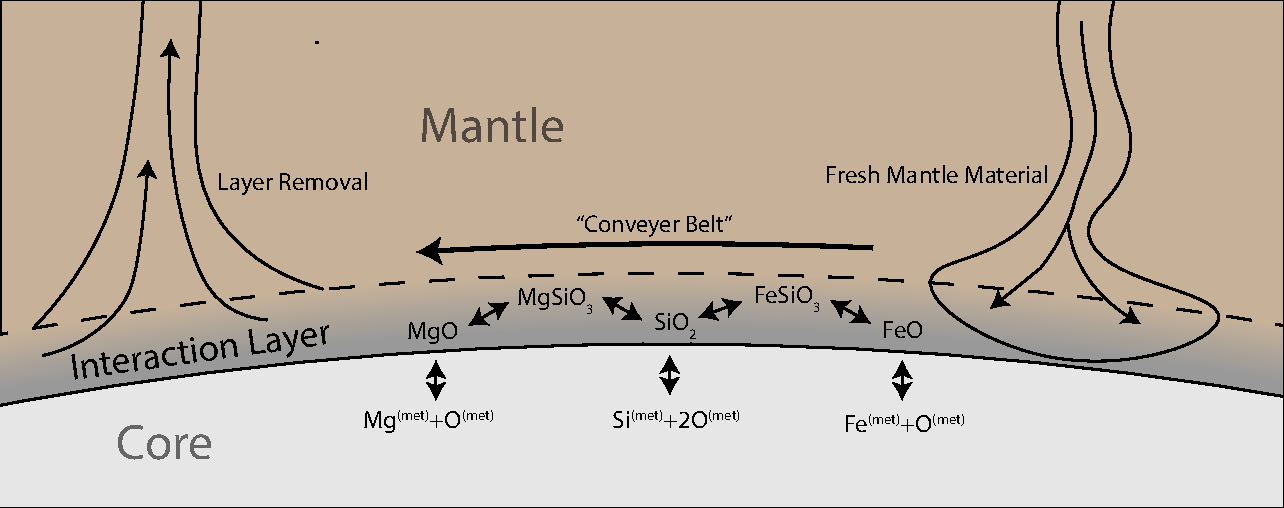
\includegraphics[width=10cm]{./figures/figure1.pdf}
		\caption{Overview of the dynamics and reactions governing chemical exchange between the core and mantle.}
		\label{fig1}
	\end{figure}
	
	To model this "conveyer belt" layer overturn, we include a layer
	erosion term in our system of differential equations that pushes each
	species towards the background mantle composition value. Assuming a
	pyrolitic background mantle composition and specifying a layer thickness
	sets the total number of moles \$M\_\{b,i\} \$ of each species \(i\) in
	the layer. Our equations are cast in terms of absolute number of moles,
	so the erosion term \(\left(\frac{dM_i}{dt}\right)_{erosion}\) for each
	species is a function only of the difference \(M_i - M_{b,i}\) and the timescale of layer overturn \(\tau\) (see supplement).
	
	In our model, we assume a present day \(\tau_p\) between 200 and 800 Myr. The early earth likely had more vigorous convection, so we set the timescale at early earth \(\tau_0 = \tau_p/8\) and set \(\tau\) at intermediate times using an exponential relationship varying between these values with a timescale of 1 Byr. 
	
	We assume a pyrolitic background lower mantle based on seismic an first-principles estimates. This consists of 83\% Bridgemanite, 16\% ferroperilase, and 1\% free SiO2, with a magnesium number of 0.8 {[}CITE{]}.
	
	\subsection{Thermodynamic Model}\label{thermodynamic-model}
	
	We model the thermodynamic evolution of Earth's core by modifying the method of \citet{Nimmo2015} to include terms for latent heat release and gravitational energy release for MgO, SiO2, and FeO exsolution. The gravitational energy and entropy released by exsolution is expressed as
	$$Q_{g,i} = \int \rho \psi \alpha_i \frac{dc}{dt}dV \, ,\qquad E_{g,i} = Q_{g,i}/T_c$$
	from Table 1 in that work. This requires an estimate of the
	compositional expansion \(\alpha_i\) for each species. We use
	\(\alpha_{MgO}\sim0.84\) (O'Rourke, Korenaga 2016) and
	\(\alpha_{SiO2}\sim1.117\) \citep{Hirose2017}. For FeO, we perform a
	simple hard-sphere estimate to compute the change in density between a
	parcel of fluid with 99 wt\% Fe, 1 wt\% O and 100 wt\% Fe to obtain
	\(\alpha_{FeO} \sim 0.28\).
	
	We compute latent heat release for each species through
	\(Q_{L,i} = L_{H,i}\frac{dm_i}{dt}\), where \(\frac{dm_i}{dt}\) is the
	change in the mass of the species with time and \(L_{H,i}\) is the
	latent heat of exsolution for each species. We use \(L_{H,SiO2} = 4300\)
	kJ/kg \citep{Hirose2017}, while \(L_{H,MgO} = L_{H,FeO}=910\) kJ/kg
	represents a value intermediate between that for SiO2 and inner-core
	solidifcation. These value has little effect on the system, as the total
	heat released by exsolution of light elements is quite small. We find \textless{}5\% difference in model run outcomes when setting all latent heat of exsolution values to zero. Note also that unlike latent heat from inner-core growth, the latent heat from exsolution does not contribute to the entropy production in the core as heat released at the CMB does not contribute to thermal convection. In fact, latent heat of exsolution has a negative effect on the energy available to power a dynamo because it decreases the core cooling rate.
	
	Chemical exchange between the core and the interaction layer at the base of the mantle causes only small changes to the bulk physical properites of the layer  and do not significantly affect mantle dynamics. Therefore, we use a simple 1D parameterized whole-mantle convection model following the method of \citep{Stevenson1983} to track the mantle temperature evolution over time. We use an Arrhenius mantle viscosity with present day viscosities varying from \(\mu_p=\) 10\(^{19.5}\) to 10\(^{21}\) Pa s. We use Stevenson's values for all parameters except for radiogenic heat production in the mantle, which we replace using the method from \citet{Korenaga2006} which includes four individual radioactive species.
	
	\subsection{Coupled Thermodynamic-Chemical System} \label{system-of-equations}
	
	We couple the chemical evolution equations and the thermodynamic model into a system of first-order ODEs. To do this, we take the derivative of each equilibrium reaction \eqref{eq:m1} - \eqref{eq:c3} with respect to temperature. These equations are tightly coupled and highly nonlinear due to the dependence of each equation on both the number of moles of each species and the total number of moles in the core or mantle. Therefore, we use the open-source sympy solver (CITE) to convert the system into a set of first-order ODEs to make solution numerically tractable. 
	
	We the thermodynamic model tracks the temperatures and the core mantle boundary and upper-mantle, while the chemical equations track the number of moles of four species in the core and five in the interaction layer. This gives a state vector $\mathbf{x}$ with eleven components. We specify the initial state by setting \(T_{CMB,0}\) and \(T_{UM,0}\) as well as the initial composition of the core \(M_{Fe}, M_{Mg}, M_{Si}, M_{O}\). This sets the initial interaction layer composition by requiring it be in equilibrium with the core at formation. We find that many initial core compositions require initial interaction layer compositions very different from what we expect at the present day. In particular, many initial compositions require a layer highly enriched in ferropericlase. Thus, we adjust the equlibrium constant governing the Bridgemanite to ferropericlase ratio towards the expected present-day value on the same timescale \(\tau\) as mantle overturn. Finally, we solve the complete system of equations forward in time from formation to the presnt day using scipy's built-in ODEint solver.
	
	\section{Results}\label{results}
	Using this model, we can compute a self-consistent evolution of the composition and thermal state of Earth's core and mantle over time. We show in figure 2 the evolution of Earth for an initial CMB temperature 5750K; initial core composition 0.5 wt\% Mg and Si, 1.5 wt\% O; interaction layer thickness 100m; present-day mantle overturn time  400 Myr; and present-day mantle viscosity 10$^{21}$Pa-s. In this history, entropy production is initially dominated by secular cooling before FeO begins to exsolve out of the core and becomes the dominant source of entropy production. Then, as the core cools, both SiO2 and MgO begin to exsolve at distinct times, causing small spikes in total entropy available but contributing less to the overall entropy budget than either FeO or secular cooling. For the $\sim$2 Byrs before inner-core nucleation, secular cooling is the largest single contributor to the entropy budget, but exsolution of light elements still produces a significant amount of entropy. Inner-core nucleation brings a powerful new source of entropy production which causes a spike in total available entropy for the dynamo and depresses the core cooling rate. This causes entropy production from cooling and exsolution to decline and allows inner-core entropy production to dominate all other sources to the present day.
	
	\begin{figure}\centering
		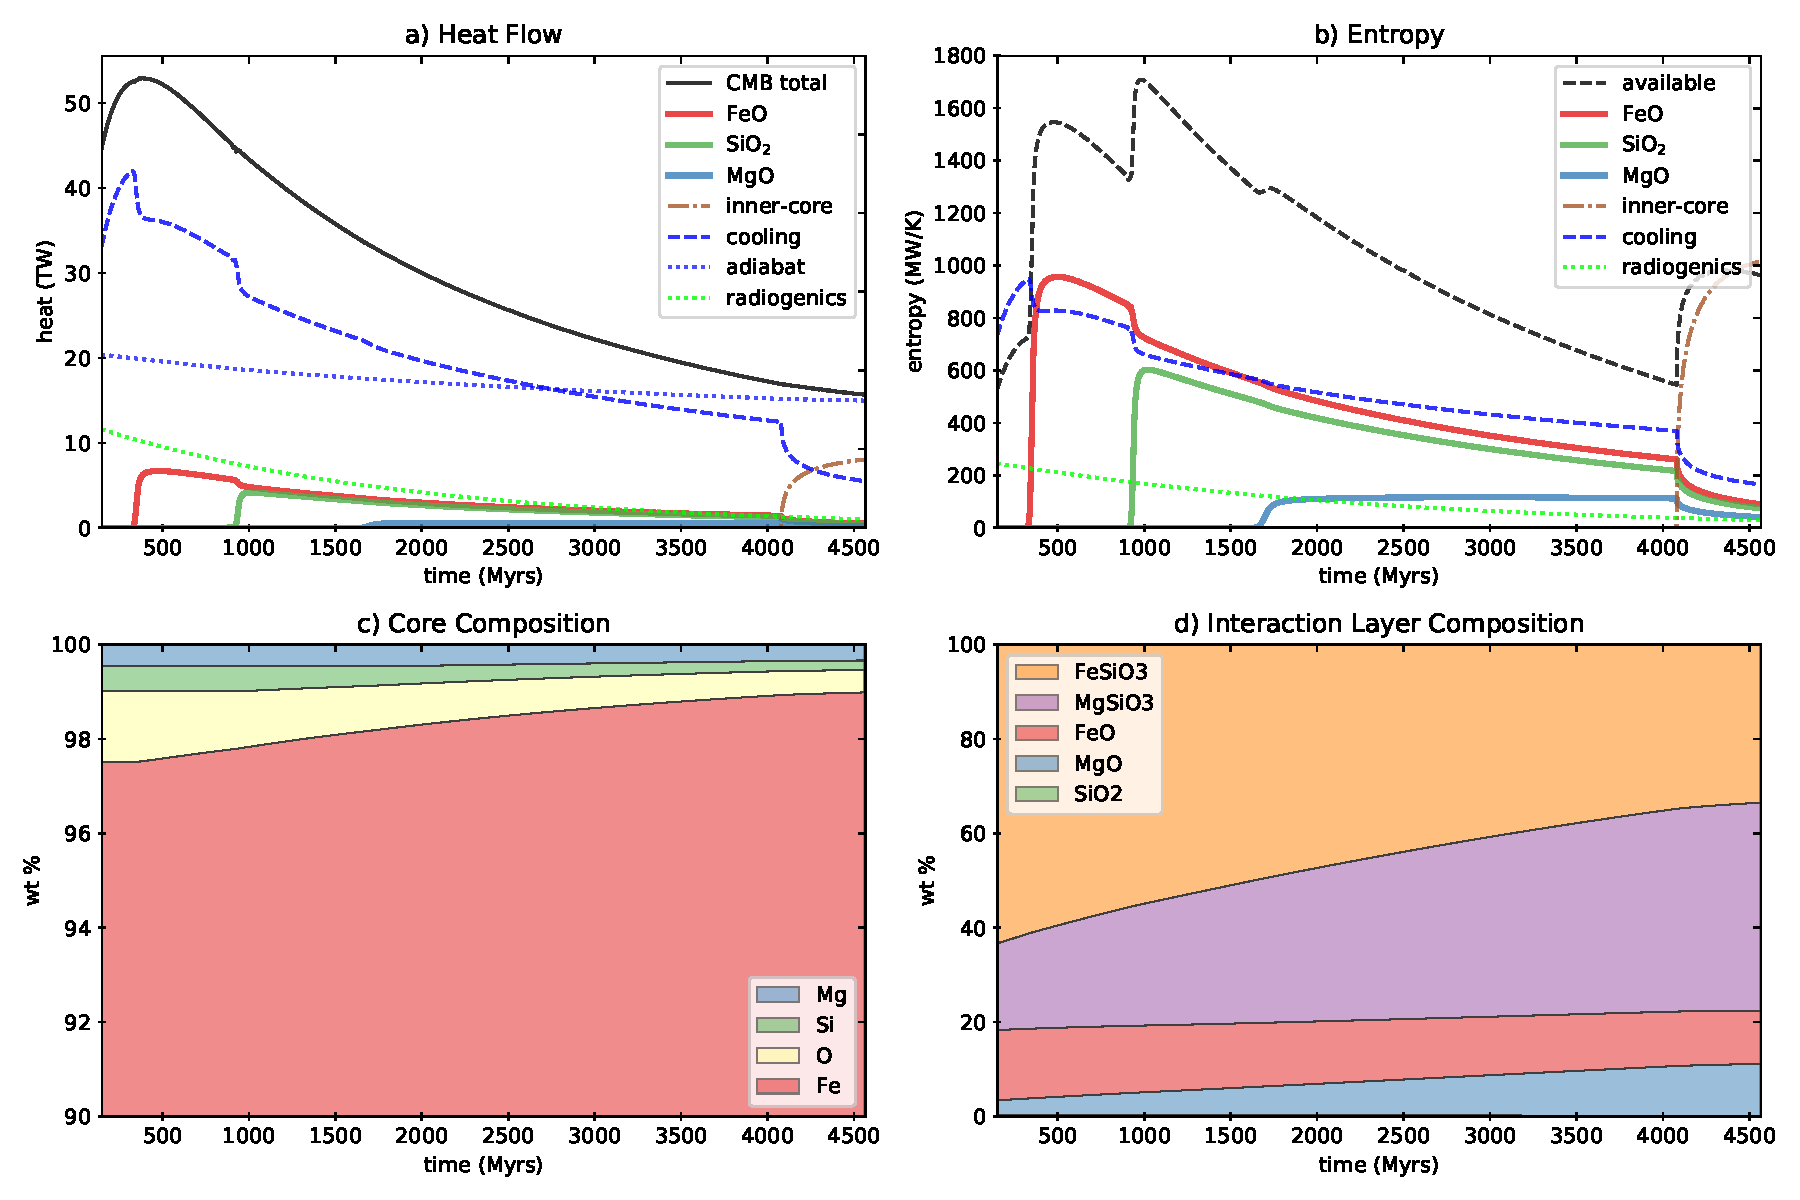
\includegraphics[width=10cm]{./figures/figure2.pdf}
		\caption{Overview of the dynamics and reactions governing chemical exchange between the core and mantle.}
		\label{fig2}
	\end{figure}
	
	In this history, the mantle interaction layer is significantly enriched in iron in the
	early Earth, with a Mg\# $\sim$ 0.25 (see fig. 2d). As exsolution slows near the present day, the enriched layer is swept away as material is incorporated from background mantle convection increasing the Mg\# to $\sim$0.6. The layer is still enriched in iron at the present	day compared to the background mantle, which has a Mg\#	$\sim$0.8. This has possible implications for the origin of LLSVPs and ULVZs, as mantle convection could collect dense material near the base of upwellings and plumes as LLSVPs or sweep material into piles to form ULVZs {[}TODO:CITE{]}. 
	
	\begin{center}\label{table:variables}
		\begin{tabular}{ l l c c}
			\multicolumn{4}{c}{Table 2: Model Variables} \\
			\hline
			Parameter & Description & Range & Units \\
			\hline
			$w_{Mg,0}$ & initial Mg wt\% in core & $10^{-5}$ - TODO & -\\
			$w_{Si,0}$ & initial Si wt\% in core		&$10^{-5}$ - TODO &-\\
			$w_{O,0}$ & initial O wt\% in core		& $10^{-5}$ - TODO&-\\
			$T_{CMB,0}$ & initial core-mantle boundary temperature & 5000 - 6250& K\\
			$H$ & interaction layer thickness& 30 - 1000 & m \\
			$\mu_p$ & present-day mantle viscosity & $10^{19.5}$ - $10^{21}$& Pa-s\\
			$\tau_p$ & present-day mantle overturn timescale	& 200 - 800 & Myrs\\
			\hline
		\end{tabular}
	\end{center}
	
	\subsection{Entropy Production Over Time}\label{entropy-production-over-time}
	We run a suite of parameters using our model, varying the values listed in table 1 and keeping runs that have result in a present-day inner-core size within
	10\% of the real value. We show entropy histories of runs that match present-day observations in figure 3. We color the histories by the dominant entropy production mechanism, with blue lines denoting secular cooling, red lines denoting FeO exsolution, and green lines denoting SiO2 exsolution. Figure 3a shows the entropy available to power a dynamo, demonstrating a huge variety of possible histories, but with some general trends visible. 
	
	Nearly all runs have FeO exsolution as the largest source of compositional entropy production, as can be seen in fig. 3b and the color of lines in fig 3a. 
	FeO exsolution produces 50-100\% of all compostional entropy in the early earth, and 40-100\% just before inner-core nucleation (figure 3b). In some histories MgO or SiO2 breifly produce more entropy that FeO, but in almost all histories FeO is the largest single source of compositional entropy production through the majority of Earth's history. However, after the inner core begins to grow, FeO
	exsolution becomes much less important, contributing less than 10\% of
	the compositional entropy budget at the present day in most histories.
	
	In general the total amount of entropy available for a dynamo is largest in the early earth, declines to a minimum in the $\sim$  billion years before inner-core nucleation, then increases suddenly with inner core nucleation and remains strong to the present day. 
	
	Secular cooling is the sole source of entropy production before inner-core nucleation, in a few histories (fig. 3c). However, even runs dominated by secular cooling usually have some amount of exsolution. Many histories show that entropy production is initially dominated by cooling before one or more elements begin to exsolve from the core and become the dominant source of entropy (see fig. 3c). Over time, cooling produces a steadily greater fraction of total entropy until it contributes 30-75\% of total entropy just before inner-core nucleation. After inner-core nucleation, it diminishes in importance and produces $\sim$15\% of total entropy at the present day.
	\begin{figure}\centering
		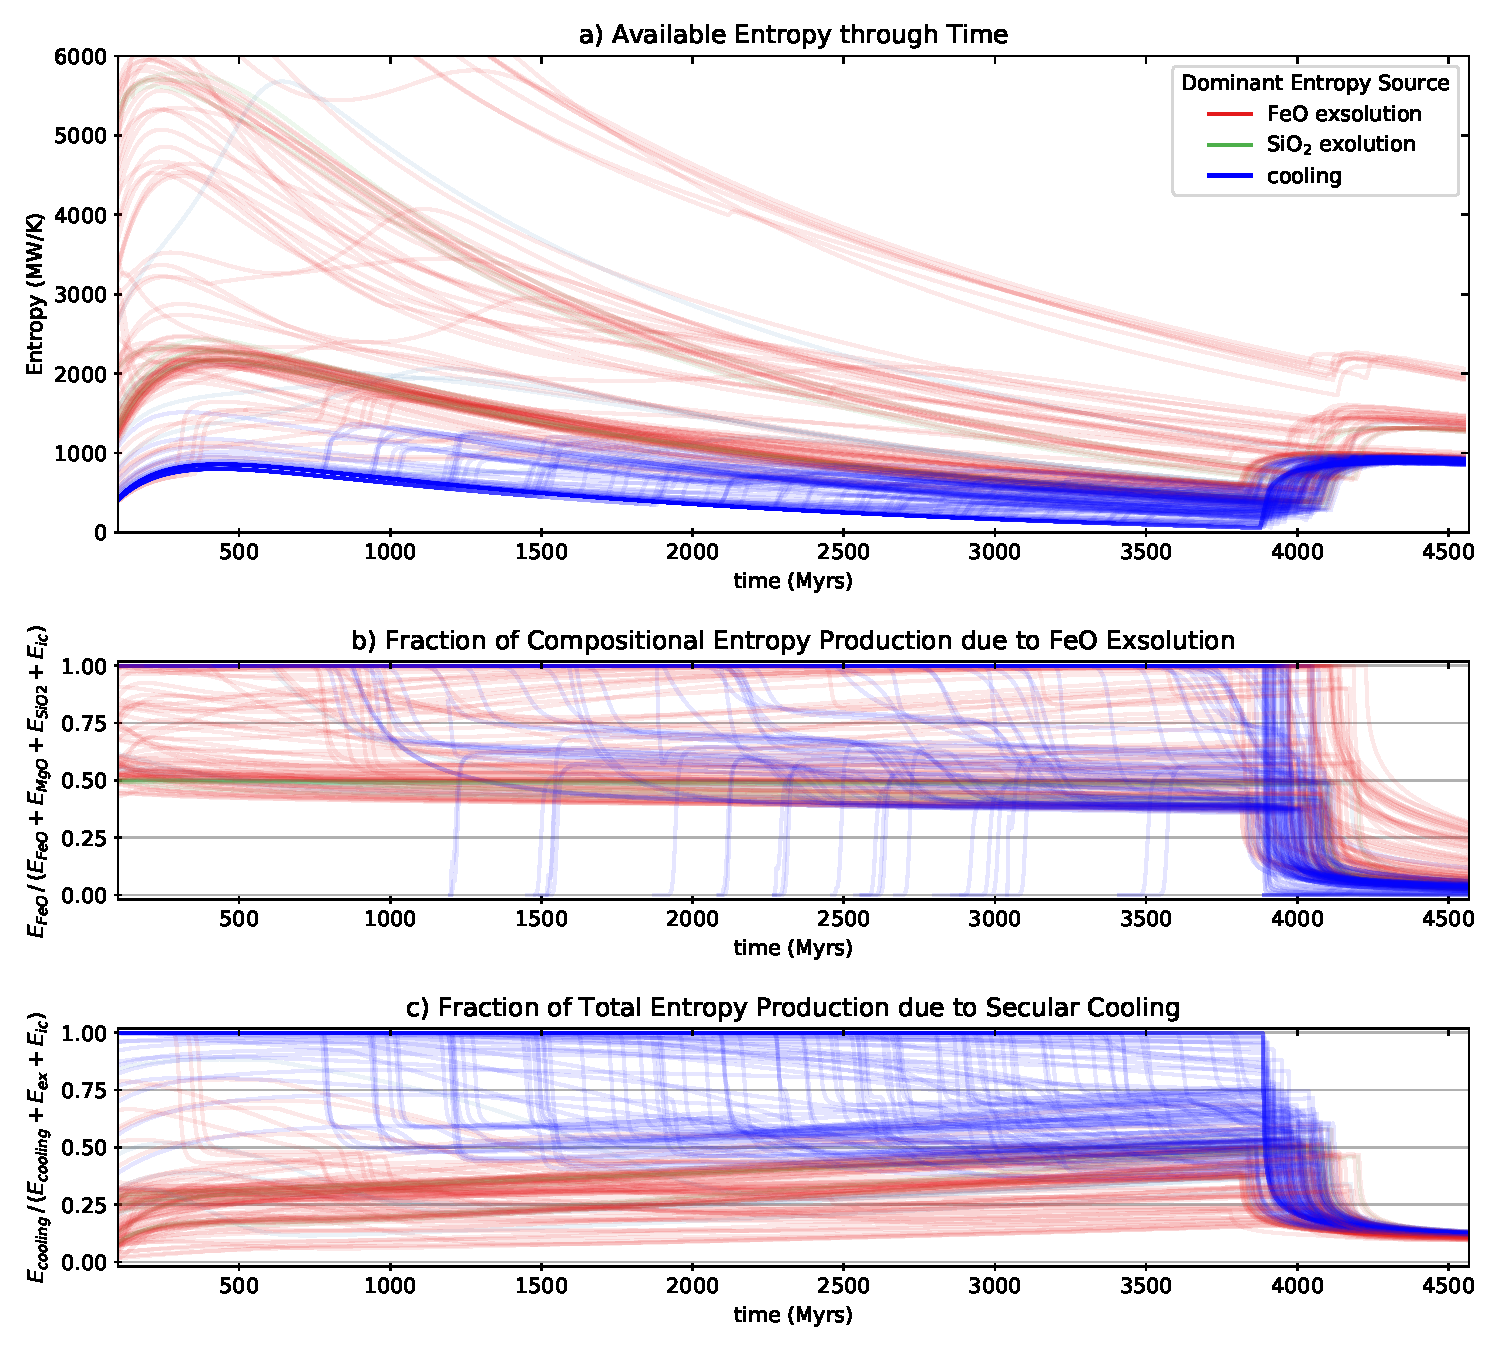
\includegraphics[width=10cm]{./figures/figure3.pdf}
		\caption{Overview of the dynamics and reactions governing chemical exchange between the core and mantle.}
		\label{fig3}
	\end{figure}
	
	\subsection{Inner-Core Nucleation}\label{inner-core-nucleation}
	We use our suite of histories to examine how exsolution affects the timing of and change in entropy production with inner core nucleation. We detail the evolution of available entropy near inner-core nucleation in fig. 4a, showing that all histories experience a positive jump in available entropy after nucleation. 
	
	The magnitude of the jump in entropy available varies between histories, and is significantly affected by the presence of exsolution. For histories with cooling as the dominant source of entropy production, the the median increase in available entropy is $\sim$ 140\%, (fig. 4b) which might be expected to produce an observable signal in paleointensity records (Olson and Christensen 2006) which many authors have searched for to constrain inner-core nucleation timing (e.g. Biggin et al. 2015). However, other authors observe a relatively constant field strength for the past 1.5 Byrs \citep{Sprain2018}, with no clear signal of inner-core nucleation. Histories with exsolution as the dominant source of entropy production in our model have an much smaller increase in entropy ($\sim$ 60\%) at inner-core nucleation, making detection in the paleomagnetic record less likely. In addition, the change in the dominant entropy production mechanism from exsolution at the CMB to inner-core growth at the center of the core might reduce the amount of entropy expressed as magnetic field observable at Earth's surface (Landeau, Aubert, Olson 2017), further reducing the size of the paleomagnetic signal. Exsolution could therefore allow a young inner core without any clear paleomagnetic signal around nucleation timing.  
	
	Exsolution also increases the variance in allowed inner-core nucleation timing (fig 4c). Dynamos powered by cooling have an inner-core nucleation ages varying from $\sim$540 to $\sim$700 Mya, with a median age of $\sim$600 Myrs. Exsolution expands the range to $\sim$350 to $\sim$760 Mya and decreases the median age to $\sim$500 Myrs. Neither of these reuslts are significantly different from those obtained by Nimmo (2015), as might be expected since we use a modified form of his core parameterization.
	
	\begin{figure}\centering
		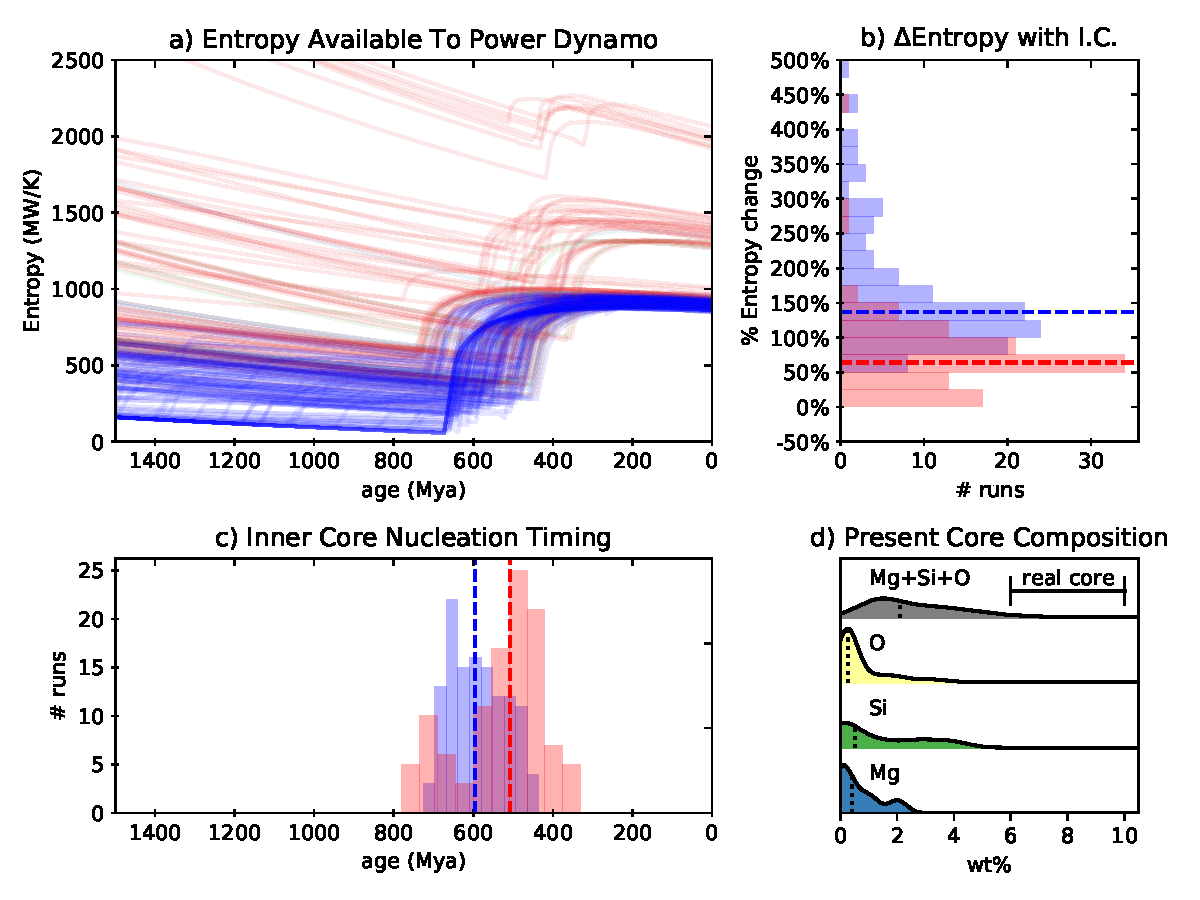
\includegraphics[width=10cm]{./figures/figure4.pdf}
		\caption{Inner-core nucleation signals and timing. (a) shows total entropy available in all valid runs, (b) is histogram of percentage increase in available entropy from 1 Myr before to 100 Myr after inner-core nucleation, with median $\sim$ 100\% increase. (c) shows a histogram of inner-core nucleation times, with median $\sim$ 600 Mya.}
		\label{fig4}
	\end{figure}
	
	\section{Conclusions}\label{conclusions}
	FeO exsolution is an important source of entropy to power Earth's
	dynamo. Exsolution of light elements from Earth's core is governed by
	the composition of the lowermost mantle and the timescale of mantle dynamics.
	
	\bibliography{citations}
	
\end{document}
